\documentclass[11pt]{article}
\usepackage[letterpaper,margin=1in]{geometry}
\usepackage{amsmath,amssymb,amsthm}
\usepackage{booktabs}
\usepackage{graphicx}
\usepackage{xcolor}
\usepackage{hyperref}
\usepackage{microtype}

\hypersetup{colorlinks=true,linkcolor=blue!55!black,urlcolor=blue!55!black,citecolor=blue!55!black}
\newtheorem{theorem}{Theorem}
\newcommand{\R}{\mathbb R}
\newcommand{\1}{\mathbf 1}

\title{A Thin-Cross Counterexample to a Star-Body Product-Section Inequality}
\author{fa\_banach\_001 / agent\_lane\_00}
\date{19 July 2026}

\begin{document}
\maketitle

\noindent\fcolorbox{red!70!black}{red!3}{%
\parbox{0.94\textwidth}{\textbf{Status: scoped candidate counterexample,
likely valid.}  The ``or even star'' strengthening in Question 12 is false.
The construction is nonconvex and does not settle the convex-body or
$L_p$, $p>2$, parts of the question.}}

\section{Source question}

Eskenazis asks the following on PDF page 13 of the source paper \cite{E}.
The paper is \emph{On extremal sections of subspaces of $L_p$},
arXiv:1806.04333.

\begin{figure}[h]
\centering

\includegraphics[width=\textwidth]{figures/open_problem_crop.png}
\caption{Question 12 as rendered from page 13 of the source paper.}
\end{figure}

The scoped clause considered here asks whether every symmetric star body
$K\subseteq\R^m$ satisfies
\begin{equation}\label{eq:source}
 |K|^{n-1}\le |K^n\cap H_\theta|
\end{equation}
for every unit $\theta\in\R^n$, where
\[
 H_\theta=\{(x_1,\ldots,x_n)\in(\R^m)^n:
 \theta_1x_1+\cdots+\theta_nx_n=0\}.
\]

\section{Proof intuition}

A very thin cross is a mixture of two perpendicular arms.  In the diagonal
section of $K^3$, three points of the cross must sum to zero.  If all three
occupy the same arm, this is possible with order-$\delta^2$ volume.  Mixed-arm
configurations are smaller, of order $\delta^3$.  The ambient normalization
$|K|^2$ is also of order $\delta^2$, but the limiting ratio is only
$27/32<1$.

The proof makes this heuristic exact.  Inclusion-exclusion writes the cross
indicator as the sum of its two rectangular-arm indicators minus their square
overlap.  Every resulting four-dimensional integral factors into two
one-dimensional interval-convolution areas, giving an explicit polynomial in
the arm thickness.

\section{The counterexample}

Fix
\[
 \delta=\frac1{100},\qquad
 H=[-1,1]\times[-\delta,\delta],\qquad
 V=[-\delta,\delta]\times[-1,1],
\]
and put $K=H\cup V\subseteq\R^2$.  Let $n=3$ and
$\theta=(1,1,1)/\sqrt3$, so
\[
 H_{\rm diag}=\{(x_1,x_2,x_3)\in(\R^2)^3:x_1+x_2+x_3=0\}.
\]

\begin{theorem}
The set $K$ is a centrally symmetric star body, and
\[
 \frac{|K^3\cap H_{\rm diag}|}{|K|^2}
 =\frac{547083}{633616}<1.
\]
Consequently, inequality \eqref{eq:source} is false for symmetric star
bodies.
\end{theorem}

\begin{proof}
\textbf{Step 1: geometric preliminaries.}
Both $H$ and $V$ are compact, centrally symmetric, convex, and contain the
origin.  Their union is therefore compact, centrally symmetric, and
star-shaped about the origin.  It contains the square
$[-\delta,\delta]^2$ in its interior, and its radial function is the maximum
of the continuous radial functions of $H$ and $V$.  Thus $K$ is a star body.
Writing $S=H\cap V=[-\delta,\delta]^2$, inclusion-exclusion gives
\begin{equation}\label{eq:area}
 |K|=|H|+|V|-|S|=8\delta-4\delta^2.
\end{equation}

The map
\[
 T:(\R^2)^2\longrightarrow H_{\rm diag},\qquad
 T(x,y)=(x,y,-x-y),
\]
has Gram matrix $\left(\begin{smallmatrix}2&1\\1&2\end{smallmatrix}\right)$ in each
coordinate.  Its four-dimensional Jacobian is therefore
$\sqrt{3^2}=3$.  Hence
\begin{equation}\label{eq:section}
 |K^3\cap H_{\rm diag}|=3I_\delta,qquad
 I_\delta=\int_{\R^2}\int_{\R^2}
 \1_K(x)\1_K(y)\1_K(x+y)\,dx\,dy.
\end{equation}

\textbf{Step 2: the interval calculation.}
For positive $a,b,c$, define
\[
 J(a,b,c)=\int_{|u|\le a}\int_{|v|\le b}
 \1_{\{|u+v|\le c\}}\,du\,dv.
\]
If $r\ge s\ge t$ is the decreasing rearrangement of $a,b,c$, slicing the
convolution of two centered intervals gives
\begin{equation}\label{eq:J}
 J(a,b,c)=
 \begin{cases}
 4st,&r\ge s+t,\\
 2(rs+rt+st)-(r^2+s^2+t^2),&r<s+t.
 \end{cases}
\end{equation}
Indeed, the first case is the plateau regime of the convolution trapezoid;
the second subtracts its two corner triangles.

Now
\[
 \1_K=\1_H+\1_V-\1_S.
\]
Expanding the three factors in \eqref{eq:section} gives 27 terms.  A term
with rectangles $R(a_1,b_1)$, $R(a_2,b_2)$, $R(a_3,b_3)$ factors as
\[
 J(a_1,a_2,a_3)J(b_1,b_2,b_3).
\]
Using \eqref{eq:J}, and grouping permutations of $H,V,S$, gives the complete
sum below; the signs include the copies of $-\1_S$.

\begin{center}
\begin{tabular}{lc}
\toprule
Grouped multisets & total contribution to $I_\delta$\\
\midrule
$HHH$ and $VVV$ & $18\delta^2$\\
$HHV$ and $HVV$ & $96\delta^3-24\delta^4$\\
$HHS$ and $VVS$ & $-72\delta^3+18\delta^4$\\
$HVS$ & $-96\delta^4$\\
$HSS$ and $VSS$ & $72\delta^4$\\
$SSS$ & $-9\delta^4$\\
\midrule
Total & $18\delta^2+24\delta^3-39\delta^4$\\
\bottomrule
\end{tabular}
\end{center}

Thus, by \eqref{eq:area} and \eqref{eq:section},
\begin{equation}\label{eq:ratio}
 \frac{|K^3\cap H_{\rm diag}|}{|K|^2}
 =\frac{3(18+24\delta-39\delta^2)}{16(2-\delta)^2}.
\end{equation}
At $\delta=1/100$, exact rational arithmetic yields
\[
 I_\delta=\frac{182361}{100000000},\qquad
 |K|=\frac{199}{2500},\qquad
 \frac{3I_\delta}{|K|^2}=\frac{547083}{633616}<1.
\]
This contradicts \eqref{eq:source}.
\end{proof}

\begin{figure}[ht]
\centering
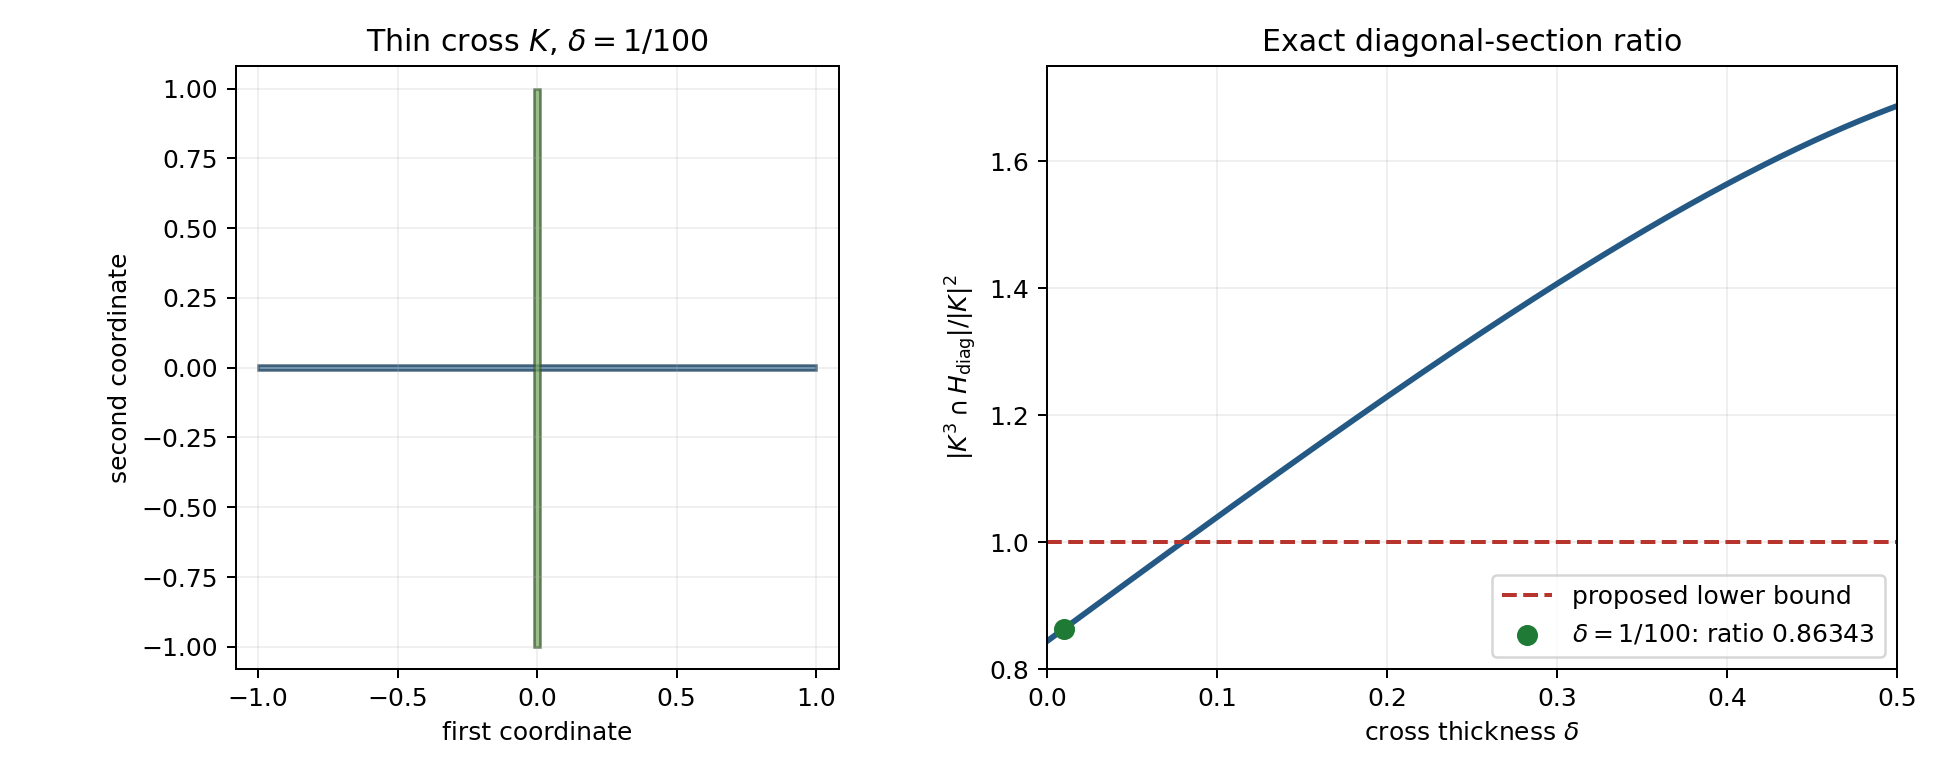
\includegraphics[width=\textwidth]{figures/thin_cross_and_ratio.png}
\caption{The thin-cross construction and its exact ratio from
\eqref{eq:ratio}.}
\end{figure}

\section{Verification}

The script \texttt{code/verify\_star\_counterexample.py} evaluates all 27
terms using rational arithmetic, confirms the polynomial for $I_\delta$ and
the final fraction exactly, and generates the figure.  It reports
\texttt{closed\_form\_match=True} and \texttt{PASS}.  Commands and output are
recorded in \texttt{verification.md}; computation is not used as a substitute
for the proof.

\section{Scope and bounded novelty check}

This theorem answers only the explicit ``or even star'' strengthening in
Question 12.  The cross is not convex.  No claim is made about symmetric
convex bodies or unit balls of subspaces of $L_p$ for $p>2$.

The run indexes were searched by arXiv id, title, question number, and core
terms.  A bounded primary-source web/arXiv search used the exact question
language, ``star body,'' ``product section,'' and ``block hyperplane.''  It
found the source and general section-volume work but no later explicit answer
or matching thin-cross calculation.  This is not an exhaustive novelty claim.

An exploratory exact-polytope search tested standard and random centrally
symmetric convex bodies in dimensions two and three and found no violation.
That finite search has no bearing on whether the convex case is true.

\section{Human-review recommendation}

Independent review should check the Jacobian factor $3$, formula
\eqref{eq:J}, and the grouped inclusion-exclusion table.  The result should
remain explicitly scoped to star bodies unless a separate convex example or
proof is found.

\begin{thebibliography}{9}
\bibitem{E}
A. Eskenazis,
\emph{On extremal sections of subspaces of $L_p$},
Discrete Comput. Geom. \textbf{65} (2021), 489--509;
arXiv:1806.04333.
\end{thebibliography}

\end{document}
